\chapter{Project Planning}
A project plan establishes project objectives, outlines activities, determines the way to accomplish goals and specifies what resources will be required - keeping in mind about the corresponding budgets and completion timeframes. A project plan specifies all of the work and steps initiated that will be done in a project and who will accomplish it.

\section{Work Breakdown Structure}
Work Breakdown Structure determines the steps that need to be initiated with a project which helps the user to accomplish strategic planning. It helps the researcher to monitor the phase of the project with an effective plan. It helps detect the risks and outbacks of the project, leading it to a more successful approach as a project planner.

\begin{figure} [H]
    \centering
    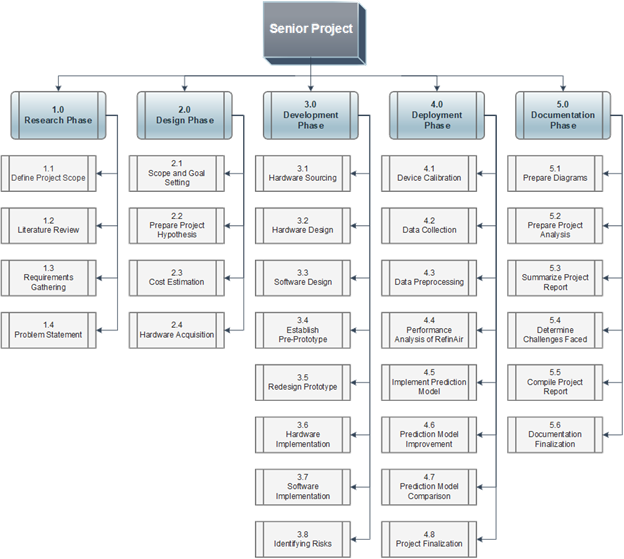
\includegraphics[width=.8\textwidth]{images/3_1_Work Breakdown Structure.png}
    \caption{Work Breakdown Structure}
    \label{fig:Work Breakdown Structure}
\end{figure}

\subsection{Air Quality Monitoring System}
\vspace{0.5cm}
This demonstrates the proposed system we aspire to make in our project. All the hardware, software implementation we want to acquire in this project will be stated here. Please note that this section contains the idea we intend to accomplish.

In this section, we will be giving insights about the steps of the project we intend to implement in order to reach our goal. In order to choose the sensors for detecting the level of air toxins, we first need to determine which air pollutants should we target to monitor. The maximum parameters need to be researched that will be appropriate for maintaining a healthy surrounding for different factors, e.g. indoor and outdoor air pollutant levels. For choosing the appropriate sensor, it is important to notice if the sensor is suitable for the environmental condition in which it will inhabitat. The range of the sensor is necessary to identify to know if the sensor will be able to give it’s best performance in terms of sensing according to the environment. The sensor shape is important because our aim is to make a compact device. 

Please note that it is important to maintain the cost estimation for cost feasibility so that normal citizens can also get the opportunity to track the rise of the catastrophe and get aware of the situation. As most of the citizens in 3rd world countries are from middle class background, this engagement in air monitoring will encourage them to use less air polluting substances or at least reduce them.

The next step to help us lead to a successful project is to read multiple research papers that are published in different Journals and Conferences related to this topic. It is advised to do a literature review before starting the project to get prepared about the upcoming steps to reach a fruitful outcome. 

After being able to choose the right sensors and other components for the project, the sensor data containing concentrations of air pollutants will be sent to the PC and simultaneously, the data will also be uploaded into the software we aspire to make. The set of data will be stored in a database and with the help of Machine Learning Algorithms our plan is to make an ‘AQI Atmospheric Map’. 


\vspace{0.5cm}
\subsubsection{3.1.1.1  Identifying requirement}
\vspace{0.5cm}
An essential step to establish the project's requirements in advance is to be inclusive about the project's requirements, which can lead to a coherent and realistic conclusion for the betterment of the society.
\begin{enumerate}

\item Identify the Stakeholders

Stakeholders are those who have a direct or indirect relationship with the organization. They are the people who make a contribution to the project in some capacity. The stakeholders of this project are the researchers whose sole aim is to run the project successfully; the machine learning engineers whose work is to input the prediction process into the system; the software engineer who makes sure to provide the customers a user friendly experience and lastly the customers who purchase the device to be aware of the alarming situation.

\item Gather information

Gathering information entails uncovering all conceivable scenarios that are important to the topic, followed by putting the best concept into action - in order to meet an effective end. This can be accomplished by reading a number of research articles and publications that are similar to the project outline. Prototypes can be created to assess which process is ideal for the project and to monitor the results. Obtaining assistance from faculty or other individuals with experience in the issue will further enlighten the researcher.

\item Verify and Validate

Time constraints can be set for each project milestone, and resources can be identified in order to complete the project as quickly as possible. Budget allocation is an important component of the project since we need to ensure that our technology is both sustainable and cost-effective because our goal is to raise awareness among people of all socioeconomic backgrounds.

\item Confirm the feasible sustainable requirements 

Multiple research and web searches on other industrial-based devices can be conducted to choose the most sustainable components for the project in order to achieve the highest level of sustainability. It is critical to learn about the drawbacks of other industrial-based gadgets so that we can add those features into our own.
\end{enumerate}

\vspace{0.5cm}
\subsubsection{3.1.1.2  Implementation}
\vspace{0.5cm}
\begin{itemize}
    \item Indoor air monitoring system
\item Outdoor air monitoring system
\end{itemize}

\subsection{Prediction Model using Satellite Data}

To cover all the regions of the country from land to water bodies for discovering the contamination level of the polluting compounds,  our goal is to extract the 550nm AOD product from the satellite and convert the 550 nm product to PM2.5 and preprocess the data. We want to prepare a scatter diagram to determine the correlation. After the correlation, we aspire to find the correct MLA to predict the area-wise PM2.5 concentration in future.

After a literature review on predicting PM2.5 from the AOD product, our main goal was to gather AOD, station PM2.5, and weather data from available online resources. We intended to collect the AOD product data from NASA EARTH DATA’s Giovanni data visualization platform. The available AOD 550 nm product was preprocessed from MODIS (Moderate Resolution Imaging Spectroradiometer) instrument aboard the Aqua Satellite, which passes from South to North poles of the earth. The obtained AOD 550 nm product is basically the level-3 atmosphere daily global product (MYD08 D3), which are derived from four level-2 MODIS AQUA atmosphere products MYD04 L2, MYD05 L2, MYD06 L2, and MYD07 L2. We selected U.S Embassy Dhaka as the region shape of the data in Giovanni. Aerosol Optical Depth 550 nm (Deep Blue, Land Only) was selected as the dataset for the AOD product. We extracted AOD data from 01-01-2017 to 31-05-2021 from the Giovanni platform. All the data was extracted as a csv file. Subsequently, PM2.5 raw concentration data were obtained from AirNow. AirNow is a partnership of the U.S EPA (Environmental Protection Agency), National Oceanic and Atmospheric Administration (NOAA), National Park Service, NASA, Centers for Disease Control, and tribal, state, and local air quality agencies. The extracted data from AirNow represents the raw concentration of PM2.5 as a unit of μg/m3. We extracted PM2.5 data from 01-01-2017 to 31-05-2021 from the AirNow website. All the data was extracted as a csv file. Afterwards, we converted the per hour data to mean concentration of PM2.5 per day to fit with the AOD 550 nm product data obtained from the AQUA MODIS. Henceforth, we obtained the weather dataset from Visual Crossing Weather services web application. The dataset contains mean temperature, rain precipitation, wind speed, visibility, cloud coverage, and humidity data. All the data are mean data of the particular day. We extracted weather data from 01-01-2017 to 31-05-2021 from the Visual Crossing Weather services website. All the data was extracted as a csv file. After successful extraction of all the datasets we combined all the datasets day-to-day from 01-01-2017 to 31-05-2021. We manually preprocessed the dataset by eliminating all the outliers and null data for any particular date. After preprocessing the dataset we split the dataset on the basis of training and testing at 70:30 ratio respectively. Afterwards, we applied multiple regression linear models and various machine learning models to predict the PM2.5 raw concentration from the AOD data. 

\emph{More to write after finalization of the prediction models.}

\vspace{0.5cm}
\subsubsection{3.1.3.1  Implementation}
\vspace{0.5cm}

\begin{itemize}
\item Predict PM2.5
\item Generate overall country AQI Atmospheric Map
 \item Cover monitoring the land and water transportation bodies.
\end{itemize}


\section{Gantt Chart}
\begin{figure} [H]
    \centering
    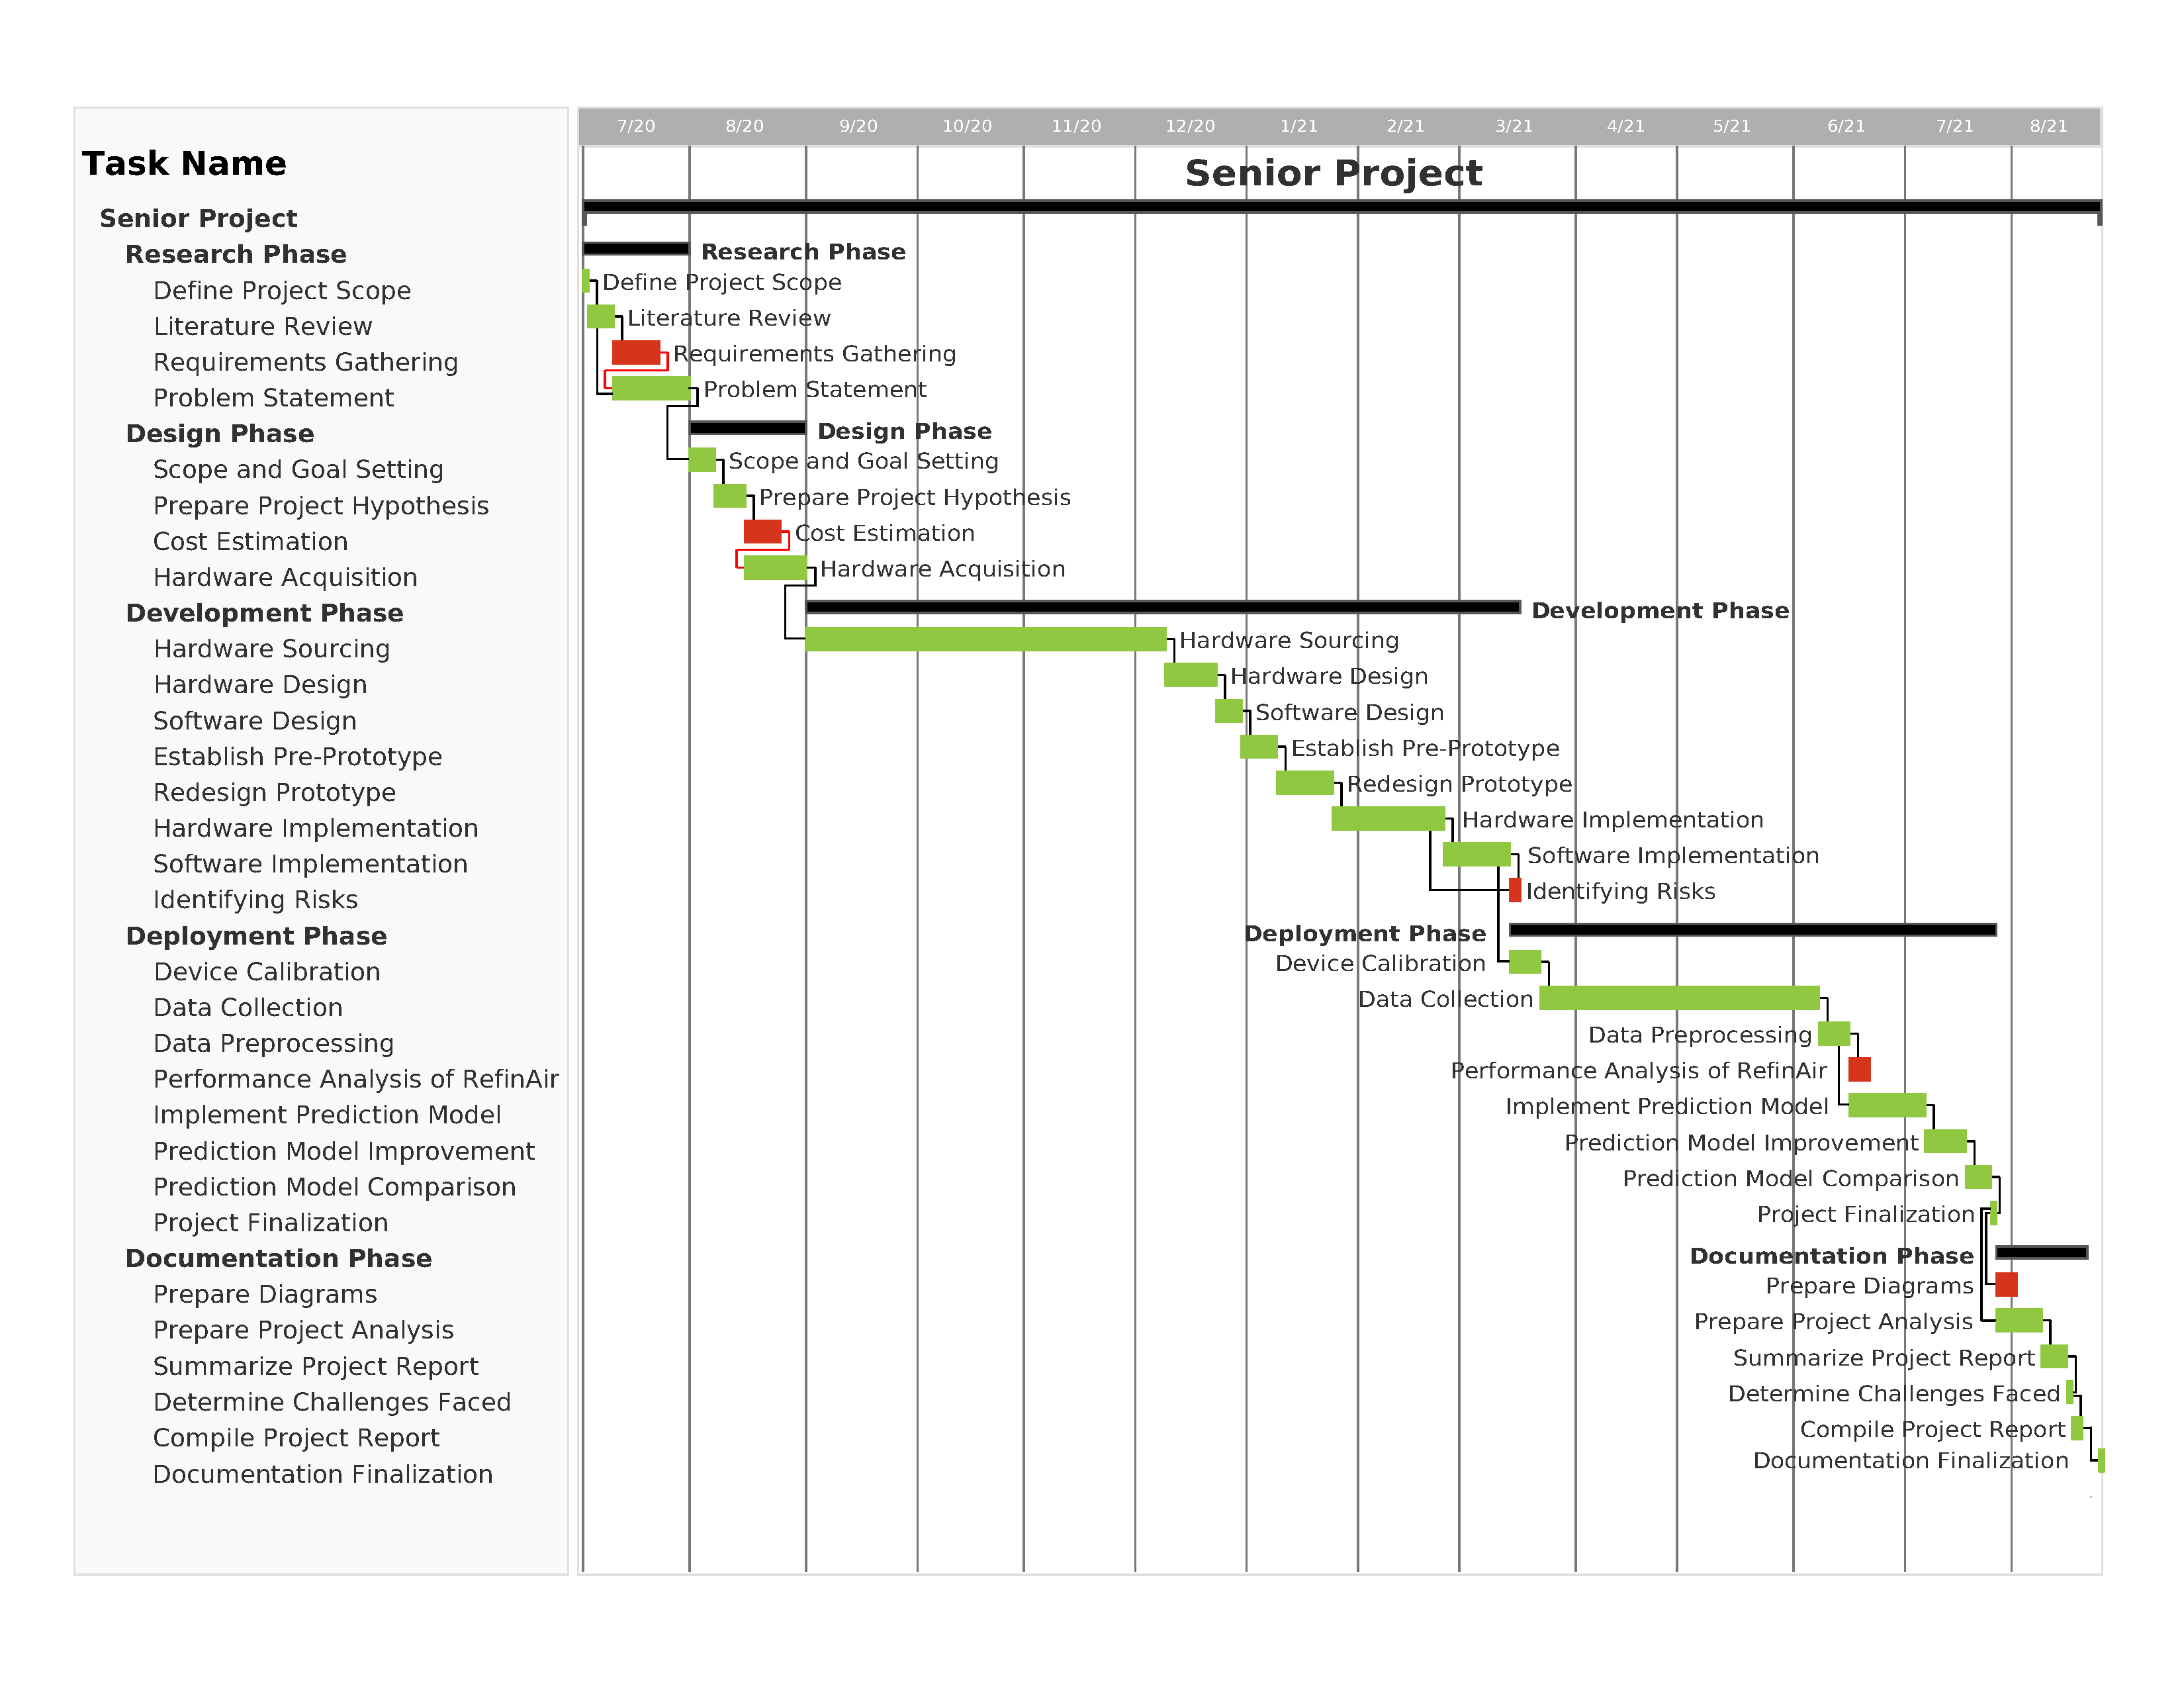
\includegraphics[width=1.1\textwidth]{images/3_2_Gantt Chart.png}
    \caption{Gantt Chart for RefinAir}
    \label{fig:Gantt Chart for RefinAir}
\end{figure}

\vspace{0.5cm}
\section{Cost Estimation}
\vspace{0.5cm}
We are offering three solutions to the problem. This section will demonstrate the component list and cost estimation of the device.

\vspace{0.5cm}
\subsection{Air Visual Pro Cost Estimation}
\vspace{0.5cm}

\vspace{0.5cm}
\subsection{RefinAir Cost Estimation}
\vspace{0.5cm}

\vspace{0.5cm}
\subsection{Research and Development Staff Cost For Prediction Model}
\vspace{0.5cm}

\vspace{0.5cm}
\subsection{Cost Estimation Scenario}
\vspace{0.5cm}
